\PassOptionsToPackage{unicode}{hyperref}
\documentclass[aspectratio=1610, 9pt]{beamer}

% Load packages you need here
\usepackage{polyglossia}
\setmainlanguage{english}

\usepackage{csquotes}
    

\usepackage{amsmath}
\usepackage{amssymb}
\usepackage{mathtools}

\usepackage{hyperref}
\usepackage{bookmark}
\usepackage[
  locale=UK,
  separate-uncertainty=true,
  per-mode=symbol-or-fraction,
]{siunitx}
\usepackage[
  backend=biber,   % use modern biber backend
  autolang=hyphen, % load hyphenation rules for if language of bibentry is not
  % german, has to be loaded with \setotherlanguages
  % in the references.bib use langid={en} for english sources
  sorting=none,
  ]{biblatex}
  \addbibresource{references.bib}  % the bib file to use
  \DefineBibliographyStrings{english}{andothers = {{et\,al\adddot}}}  % replace u.a. with et al.
  
  
% load the theme after all packages
\usetheme[
  showtotalframes, % show total number of frames in the footline
]{tudo}

% Put settings here, like
\unimathsetup{
  math-style=ISO,
  bold-style=ISO,
  nabla=upright,
  partial=upright,
  mathrm=sym,
}
\setbeamertemplate{caption}{\raggedright\insertcaption\par}

\title{Determining the dielectric function through THz-Transmission measurments}
\author[M.~Koch]{Max Koch}
\institute[AG Wang]{Group Wang \\  faculty Physics}
%\titlegraphic{\includegraphics[width=0.3\textwidth, angle=90]{images/setup.jpeg}}


\begin{document}

\maketitle

\section{Goal}
\begin{frame}
Goal: determine the refractive index \
\begin{equation}
  n_s = n - i\kappa
\end{equation}
with real part $n$ and complex part $\kappa$ of the refractive index.
Then determine the dielectric function 
\begin{equation}
  \epsilon = \epsilon_1 - i\epsilon_2 = n_s ^2
\end{equation}
of which
\begin{equation}
  \epsilon_1 = n^2 - \kappa^2
\end{equation}
and 
\begin{equation}
  \epsilon_2  = 2n\kappa 
\end{equation}
if the material is nonmagnetic.\\
\textcolor{tugreen}{Fundamentals of measurement in terahertz time-domain spectroscopy} from Withayachumnankul, J Infrared Millim Terahertz Waves, \textbf{35} (2014) 
\end{frame}

\begin{frame}
  Additional one can calculate the optical conductivity \
  \begin{equation}
    \sigma_s  = \sigma_1 - i \sigma_2 
  \end{equation}
  from the real part of the refractive index 
  \begin{equation}
    \sigma_1 = \frac{n \kappa \omega}{2\pi}
  \end{equation}
  aswell as the complex part of the optical conductivity from the complex part of the refractive index
  \begin{equation}
    \sigma_2 = \left( 1 - n^2 - \kappa^2\right) \frac{\omega}{4\pi}
  \end{equation}
  \textcolor{tugreen}{Electrodynamics of Solids: Optical Properties of Electrons in Matter} from Dressel, M. and Grüner, G. Cambridge University Press, \textbf{2} (2002) 
\end{frame}

\section{Scheme}
\begin{frame}{Scheme}
  Lets take a look at the experimental scheme\\
  \begin{center}
    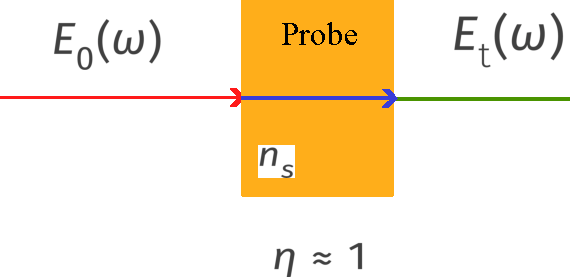
\includegraphics[width=0.5\textwidth]{images/Transmission.pdf}
\end{center}
The incoming THz-pulse $E_0(\omega)$ gets diffracted two times, and is transmitted as wave $E_\text{t}(\omega)$.
We assume an incident angel of $\theta=\SI{0}{\degree}$.
All reflections are neglected.
The refractive index of the probe is $n_s$, its length is set to be $l$.
The refractive index of the surrounding medium is $\eta$ in case of air $\eta\approx 1$.\\
\textcolor{tugreen}{Far-infrared time-domain spectroscopy with terahertz beams of dielectrics and semiconductors} from D. Grischkowsky, J. Opt. Soc. Am. B \textbf{7} (1990).
\end{frame}

\begin{frame}{Transmitted wave}
  The transmitted wave is defined as 
  \begin{equation}
    E_\text{t}(\omega) = t(\omega) E_0(\omega)
  \end{equation}
  where
  \begin{equation}
    t(\omega) = \tau \tau' \symup{exp}\left[- i n_s(\omega) \frac{\omega l }{c}\right]
  \end{equation}
  is the transmission coeffiecient.
  The complex transmission coeffiecients 
  \begin{align}
    \tau = & \frac{2}{1 + n_s} \\
    \tau' = &  \frac{2 n_s}{1+ n_s} 
  \end{align}
  are dependent on the refractive index $n_s$.
\end{frame}

\begin{frame}
  Lets do a first summary of our assumptions so far:
  \begin{itemize}
    \item No reflections
    \item Incident angle of $\theta=\SI{0}{\degree}$
    \item The probe is completly homogenous
  \end{itemize}
  with those assumptions the transmitted wave can be written as 
  \begin{equation}
    E_\text{t}(\omega) = \eta\frac{4 n_s (\omega)}{(n_s(\omega) + 1)^2} \symup{exp}\left[ -i n_s (\omega) \frac{\omega l }{c}\right] E_0(\omega)
  \end{equation}
\end{frame}

\begin{frame}{References measurment}
  The references wave 
  \begin{equation}
  E_\text{ref}(\omega) = \eta \symup{exp}\left[ -i \frac{\omega l }{c}\right] E_0(\omega)  
  \end{equation}
  differs from the original THz-pulse $E_0(\omega)$ as it travels some distance $l$.
  \begin{center}
  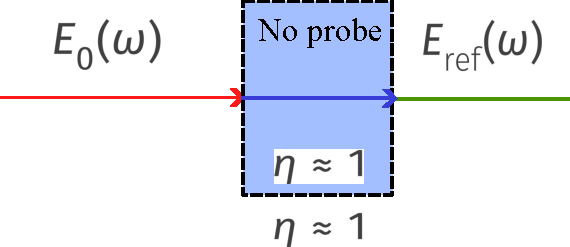
\includegraphics[width=0.5\textwidth]{images/reference.pdf}
  \end{center}
\end{frame}

\section{Complex transfer function}
\begin{frame}{Complex transfer function}
  We define the complex transfer function 
  \begin{equation}
    H_0(\omega) = \frac{E_\text{t}(\omega)}{E_\text{ref}(\omega)}
  \end{equation}
  can be defined.
  After plugging in the definitions of $E_\text{t}(\omega)$ and $E_\text{ref}(\omega)$, $H_0(\omega)$ yields
  \begin{equation}
    H_0 (\omega) = \frac{4 n_s(\omega)}{(n_s(\omega) +1)^2} \symup{exp}\left[-\kappa(\omega) \frac{\omega l }{c}\right] \symup{exp}\left[-i (n (\omega) - 1) \frac{\omega l}{c}\right]
  \end{equation}
  \end{frame}

\begin{frame}{Extracting phase}
  We can't solve $H_0$ analyticly, leaving us with two options.
  One way is to assume that $n_s \approx n$.\\
  This simplifies to 
  \begin{equation}
    H(\omega) = \frac{4n(\omega)}{(n(\omega) + 1)^2} \symup{exp}\left[-\kappa(\omega) \frac{\omega l }{c}\right] \symup{exp}\left[- i(n(\omega) - 1) \frac{\omega l}{c}\right]
  \end{equation}
  of which the phase
  \begin{equation}
    \Phi(H(\omega)) = -[n(\omega) - 1] \frac{\omega l}{c}
  \end{equation}
  and the logarithm is
  \begin{equation}
    \symup{ln}|H(\omega)| = \symup{ln}\left[ \frac{4n(\omega)}{(n(\omega) +1)^2}\right] - \kappa(\omega) \frac{\omega l}{c} \, .
  \end{equation}
alternatively Numerical approximations can be used.\\
\textcolor{tugreen}{Fundamentals of measurement in terahertz time-domain spectroscopy} from Withayachumnankul, J Infrared Millim Terahertz Waves, \textbf{35} (2014)\\
\textcolor{tugreen}{A reliable method for extraction of material parameters in terahertz time-domain spectroscopy} from Duvillaret, IEEE, \textbf{2} (1996)
\end{frame}

\section{Numerical approximation}
\begin{frame}{Numerical approximation}
  If disregarding $\kappa$ is no option, the numerical sultion needs to be employed.
  To do so we define a root finding problem 
  \begin{equation}
    \Delta(H(\omega)) \overset{!}{=} 0 = H_0(n, \kappa, \omega) - H_\text{meas}(\omega)
  \end{equation}
  However, this root finding problem isn't smooth nor monotonous.
  To overcome this problem we define a error function 
  \begin{equation}
    \delta(n, \kappa) = \delta \phi^2 + \delta \rho^2
  \end{equation}
  with the two variables 
  \begin{align}
    \delta \phi(\omega) &= \symup{ln}(\left| H_0(\omega, n , \kappa)\right|) - \symup{ln}(\left| H_\text{meas}(\omega, n , \kappa)\right|) \\
    \delta \rho(\omega) &= \Phi(H_0(\omega, n , \kappa)) - \Phi(H_\text{meas}(\omega, n , \kappa))
  \end{align}
  where $\Phi(H(\omega))$ is the phase of the Transferfunction.
\end{frame}

\begin{frame}{Linearization and unwrapping of phase}
  % I need to minimize text here and put some more figures.
  % for now its just so that I dont forget what I want to say at this slide.
  \begin{columns}
    \begin{column}{0.4\textwidth}
      The phase $\Phi(H_0(\omega, n, \kappa))$ of the Transferfunction has to be extracted.
      Should be linear and homogenous.
      But it varies between $-\pi$ and $\pi$. And noise makes it sometimes hard to unwrap.\\
      To make it continous, the values need to be $2\pi$ shifted every time a phase jump would occure.
      So we approximation the phase by a linear function and shifted to cross zero as $\omega=0$.\\
      We are left with a linear phase $\Phi_\text{lin}(T_\text{meas}(\omega, n, \kappa))$.
    \end{column}
    \begin{column}{0.6\textwidth}
      \begin{figure}
        \only<1>{\centering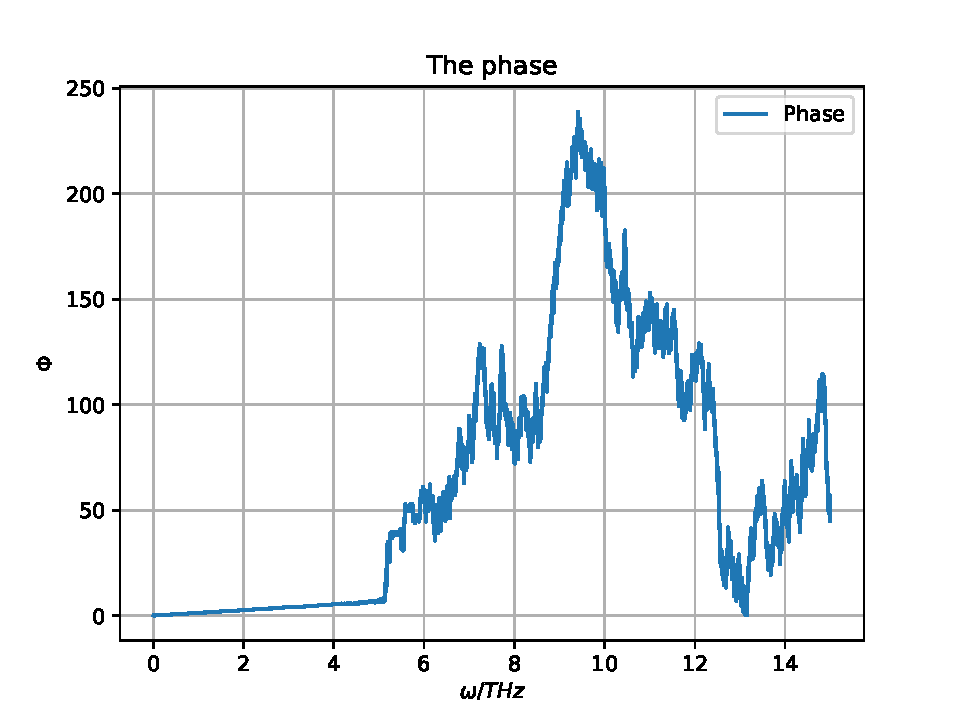
\includegraphics[width=0.8\textwidth]{images/THzPhase.pdf}}
        \only<2>{\centering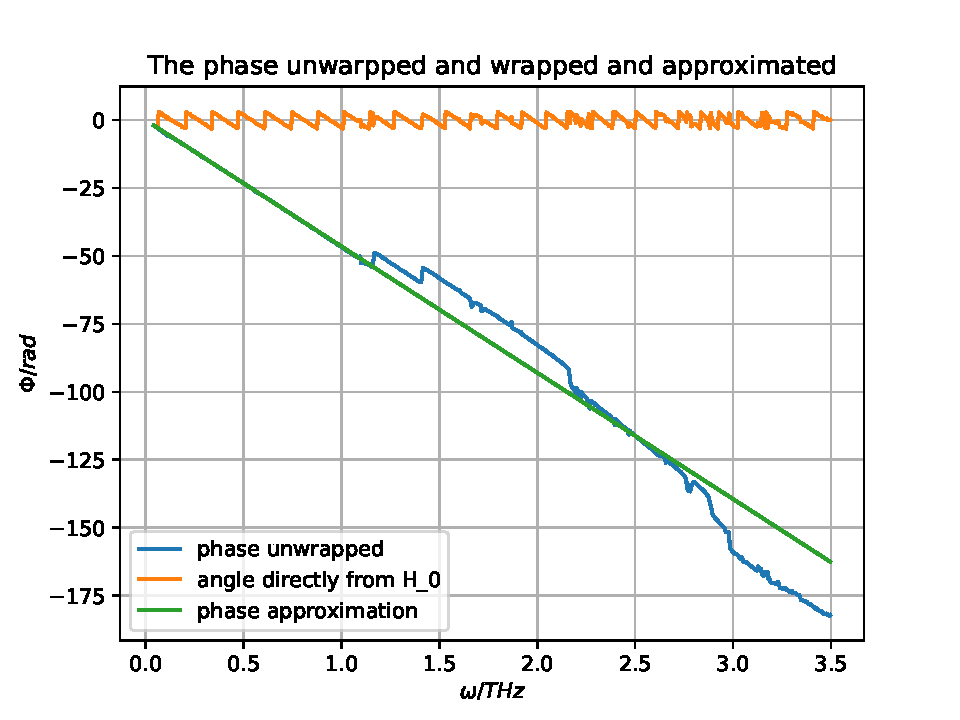
\includegraphics[width=0.8\textwidth]{images/THzPhase_approximation.pdf}}
      \end{figure}
    \end{column}
  \end{columns}
\end{frame}

\begin{frame}{Minimizing the error function}
  Now we can start to minimize $\delta(n, \kappa)$.
  From its definition one can see that it's formulated like a paraboloid.
  \begin{equation}
    \delta(n, \kappa) = \delta \phi^2 + \delta \rho^2
  \end{equation}
  \begin{equation}
    \delta(n, \kappa) = \delta(\vec{r}) = \frac{1}{2} \vec{r} A\vec{r} - \vec{b} \vec{r} + c
  \end{equation}
  where $\vec{r} = \begin{pmatrix} n\\ \kappa \end{pmatrix}$ defines the position on the plane.
  This means if one can find the $\vec{r}_{min}$ that corresponds to the minimum value of the paraboloid a good solution to
  \begin{equation}
    \Delta(H(\omega)) \overset{!}{=} 0 = H_0(n, \kappa, \omega) - H_\text{meas}(\omega)
  \end{equation}
  is found.
\end{frame}

\begin{frame}
  \begin{columns}
    \begin{column}{0.5\textwidth}
      \begin{centering}
        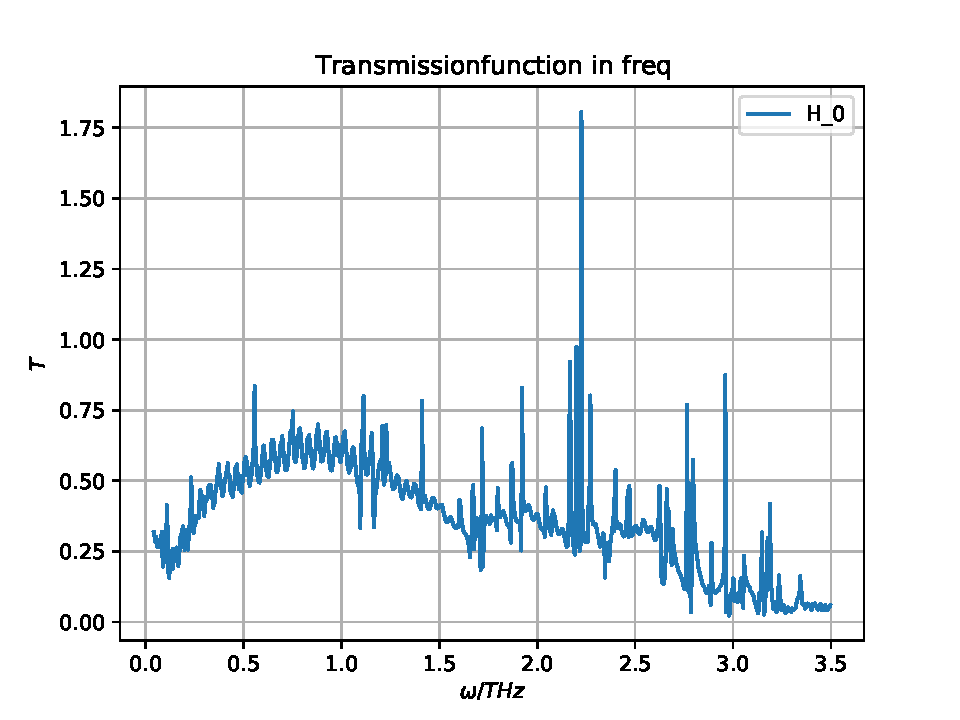
\includegraphics[width=\textwidth]{images/Transmissionfunction.pdf}
        {The transferfunction for ZnTe.}
      \end{centering}
    \end{column}
    \begin{column}{0.5\textwidth}
      \begin{centering}
        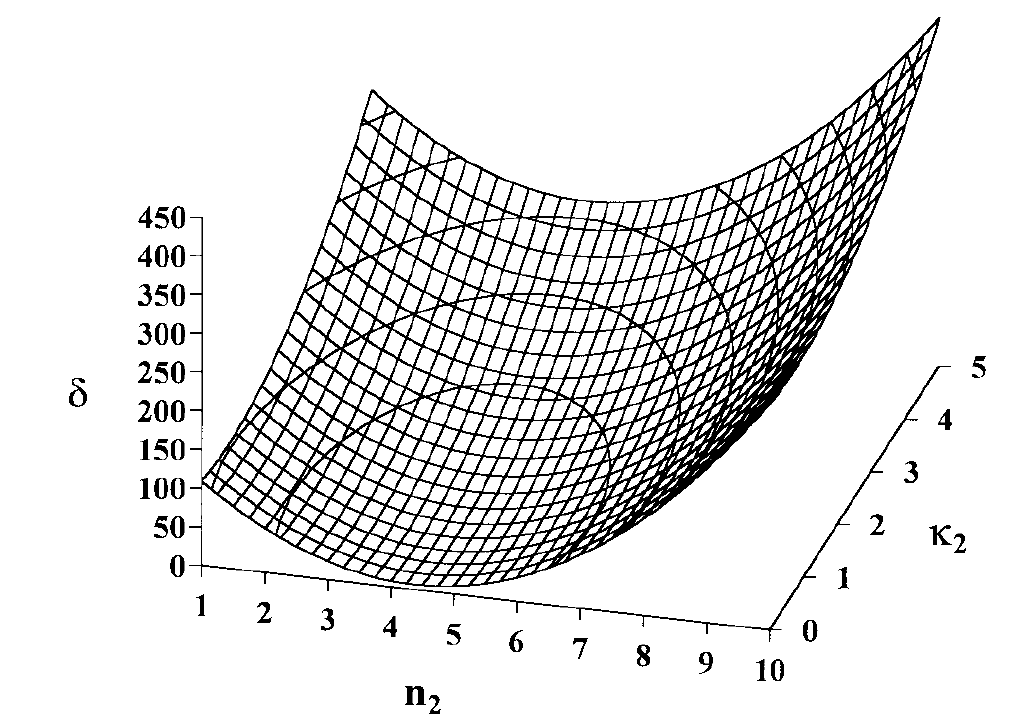
\includegraphics[width=\textwidth]{images/delta.png}
        {The deltafunction for one $\omega$ and some testvalues for $H_\text{meas}$.}
      \end{centering}
    \end{column}
  \end{columns}
\end{frame}

\begin{frame}
  There are several ways to minimize a two dimensonial function. The most common would be the Newton-Raphson-method
  \begin{equation}
    \vec{r}_{p + 1} = \vec{r}_{p} - H^{-1}(n,\kappa)\cdot\vec{\nabla}\delta(n, \kappa) \, .
  \end{equation}
  However, this algorythm doesn't work with boundaries and as $n \geq 1$ its usually faster to use a different algorythm.
  I choose to use the $L-BFGS-B$ as an easy to use python implementation already exists, it considers bounds and is usually faster than the Newton-Raphson-method.
  In any case a solution $\vec{r}_{min}$ should be found after a few iterations.
  If the sultion $\vec{r}_{min}$ for one frequency $\omega$ is determined  we can move on to the next.
  Usually it's best to start from high frequency and move down to low as the noise is lower at high frequencies.
  The determined value $\vec{r}_{min}$ from the previous step, is used as starting point for the next minimization.\\
  \textcolor{tugreen}{A Limited Memory Algorithm for Bound Constrained Optimization} from Byrd, Richard H., SIAM, \textbf{16} (1995)
\end{frame}

\begin{frame}{Thick sample solution}
  To summarize the steps we already took:
  \begin{itemize}
    \item[1.] Measure probe and reference data 
    \item[2.] Calculate Transferfunction $H_0(\omega)$
    \item[3.] Determine the phase $\Phi(H_\text{meas}(\omega, n, \kappa))$
    \item[4.] Linearise phase
    \item[5.] Minimize $\delta(\omega, n, \kappa)$ starting from high frequencies
    \item[6.] Use solution of previous step $\vec{r}_{min}$ as starting point for next step 
  \end{itemize}
\end{frame}

\section{Thin samples}
\begin{frame}{Thin sample solution}
As optically thin samples reflect the THz-wave and transmitt it after a whole pass they need to be treated different.\\
To take these reflections into account we have to cosider some additional effects.\\
These effects are caused by the Farby-Perot factor.
\end{frame}

%\begin{frame}{Determining the refractive index}
%  We can now determine $n$ and $\kappa$
%  \begin{equation}
%    n(\omega) = 1 - \frac{c}{\omega l} \Phi(H(\omega))
%  \end{equation}
%  and the complex refractive index 
%  \begin{equation}
%    \kappa(\omega) = \frac{c}{\omega l } \left( \symup{ln}\left[ \frac{4 n(\omega)}{(n(\omega) + 1)^2}\right] - \symup{ln}|H(\omega)|\right)
%  \end{equation}
%  from which the absorption coeffiecient
%  \begin{equation}
%    \alpha(\omega) = \frac{2 \omega \kappa(\omega)}{c}
%  \end{equation}
%  can be calculated.
%  Note that a special unwrapping process is necessary to determine $\Phi(H(\omega))$, in python \textit{numpy.unwrap()} can be used to do this.
%\end{frame}

%\begin{frame}{Example data}
%  By using the discussed methods a reference dataset is analyzed.
%  The measured data is plotted below 
%  \begin{center}
%    \begin{columns}
%      \begin{column}{0.5\textwidth}
%        \begin{figure}
%          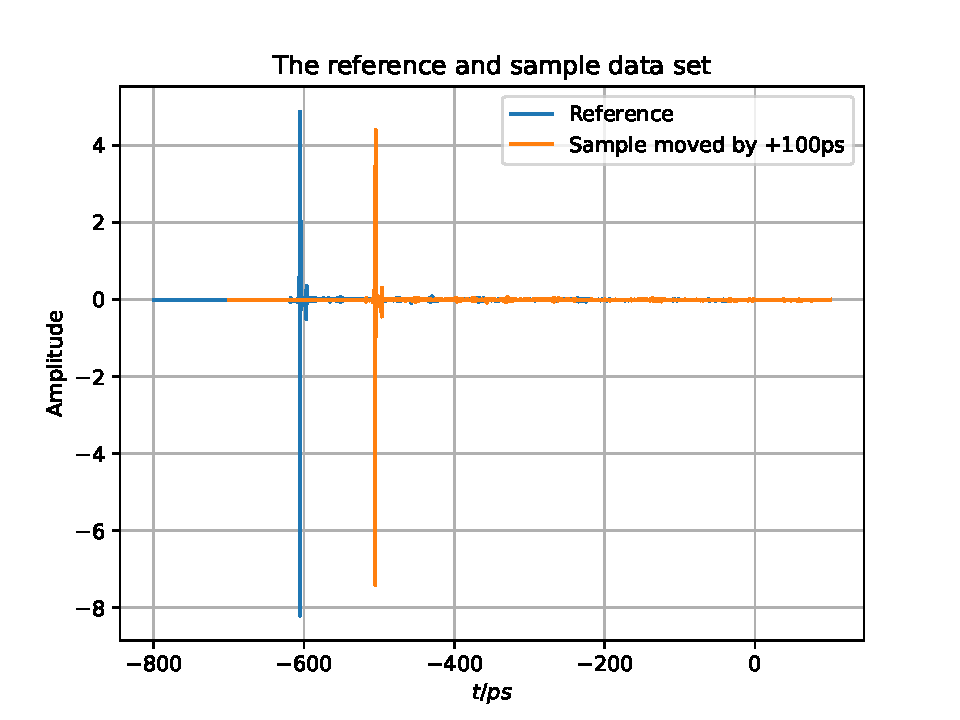
\includegraphics[width=0.8\textwidth]{images/THz1.pdf}
%          \caption{Some transmission data of Teflon foil, with a thickness of $\SI{0.25}{\milli\meter}$.}
%        \end{figure}
%      \end{column}
%      \begin{column}{0.5\textwidth}
%        \begin{figure}
%          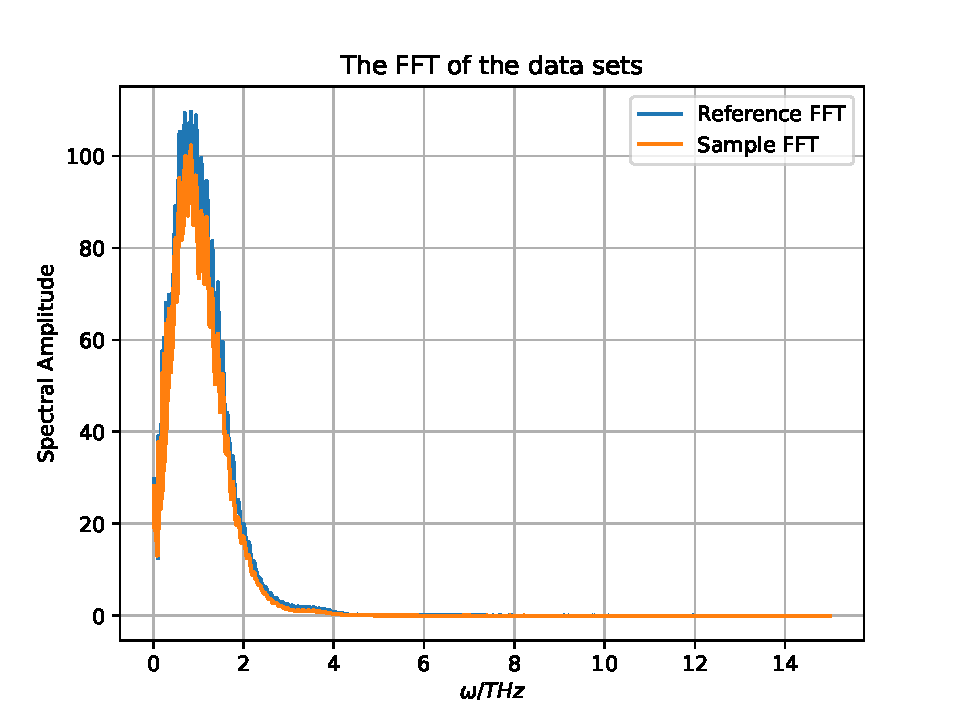
\includegraphics[width=0.8\textwidth]{images/THz4_1.pdf}
%          \caption{The FFT of the transmission data of Teflon foil, with a thickness of $\SI{0.25}{\milli\meter}$.}
%        \end{figure}
%      \end{column}
%    \end{columns}
%  \end{center}
%\end{frame}

%\begin{frame}{Refractive index}
%  The refractive index is then determined by the Quotient of Transmission and reference data in frequency space.
%  \begin{equation}
%    n(\omega) = 1 - \frac{c}{\omega l} \Phi(H(\omega))
%  \end{equation}
%  The result can be seen below:
%  \begin{center}
%    \begin{figure}
%      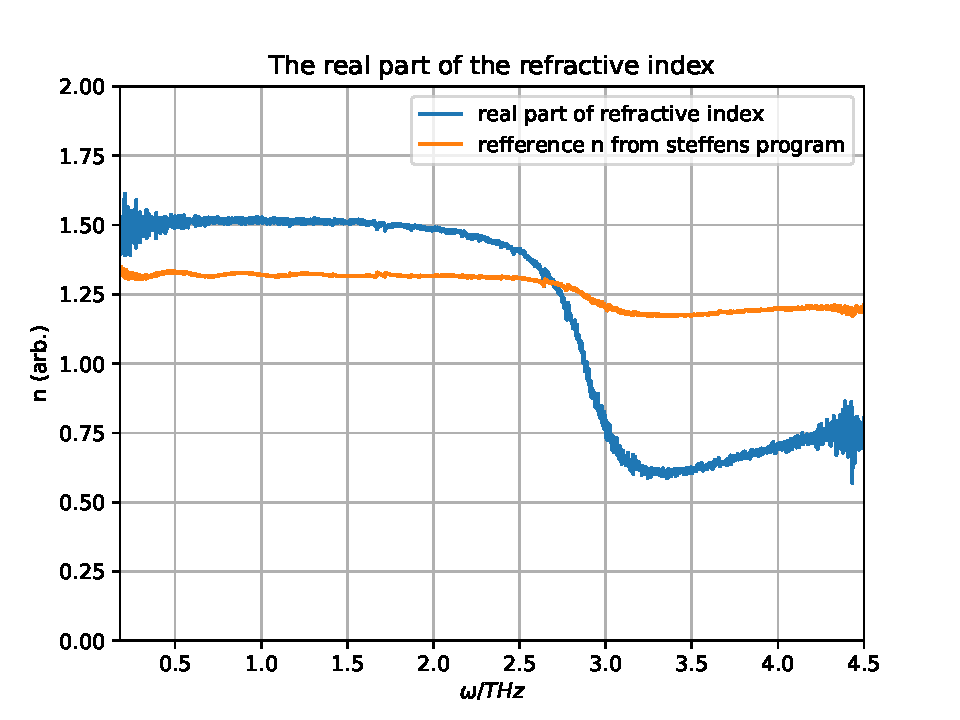
\includegraphics[width=0.5\textwidth]{images/THz5_1.pdf}
%      \caption{The refractive index of Teflon as calculated by the equation shown above.}
%    \end{figure}
%  \end{center}
%\end{frame}

%\begin{frame}{Absorption coeffiecient}
%  The absorption coeffiecient is then determined by
%  \begin{equation}
%    \alpha(\omega) = \frac{2 \omega \kappa(\omega)}{c}
%  \end{equation}
%  where $\kappa$ is the complex refractive index, which is determined by 
%  \begin{equation}
%    \kappa(\omega) = \frac{c}{\omega l } \left( \symup{ln}\left[ \frac{4 n(\omega)}{(n(\omega) + 1)^2}\right] - \symup{ln}|H(\omega)|\right)
%  \end{equation}
%  The result can be seen below:
%  \begin{center}
%    \begin{figure}
%      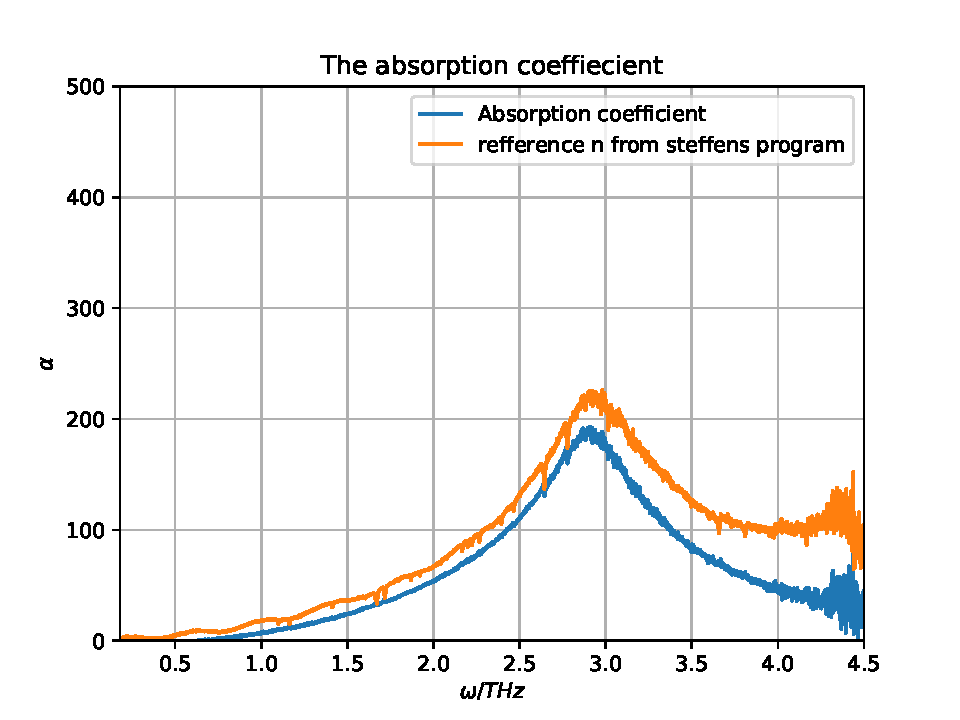
\includegraphics[width=0.4\textwidth]{images/THz6.pdf}
%      \caption{The absorption coeffiecient of Teflon as calculated by the equation shown above.}
%    \end{figure}
%  \end{center}
%\end{frame}

%\begin{frame}{Phase}
%  Just as a reference we can also plot the phase.
%  The result can be seen below:
%  \begin{center}
%    \begin{figure}
%      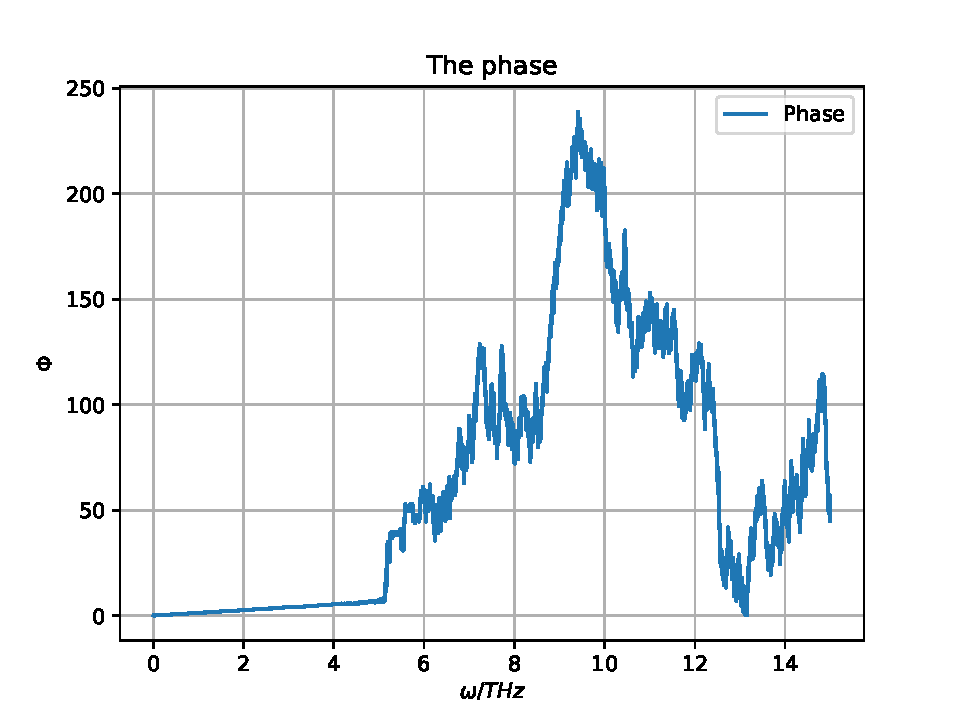
\includegraphics[width=0.5\textwidth]{images/THzPhase.pdf}
%      \caption{The Phase of Teflon as calculated by the equation shown above.}
%    \end{figure}
%  \end{center}
%\end{frame}

\begin{frame}{Fabry-Perot factor}
  Now lets take a look at the reflections inside the probe.
  The fresnel equations tell us that for every additional path that the wave takes inside the medium we have to multiply it by 
  \begin{equation}
    \rho'^2 = \left(\frac{1 - n_s}{1 + n_s}\right)^2
  \end{equation}
  aswell as a phase shift factor 
  \begin{equation}
    \Phi = \symup{exp}\left[-k \cdot i n_s \frac{\omega l}{c}\right]
  \end{equation}
  where $k$ is the number transmissions inside the probe.
  \begin{figure}
    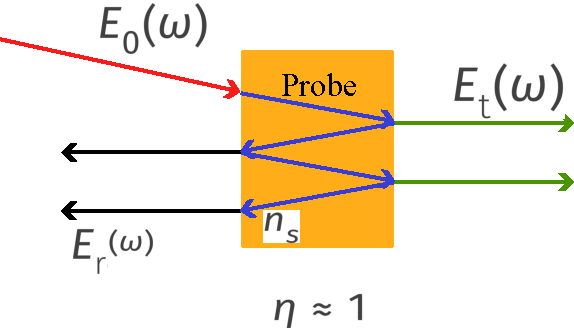
\includegraphics[width=0.4\textwidth]{images/Perot.pdf}
    \caption{Through reflections inside the medium the transmitted wave $E_\text{t}(\omega)$ will consist of several phase shifted reflections.}
  \end{figure}
\end{frame}

\begin{frame}
  If we consider all the reflections inside the probe the transmitted wave will look like
  \begin{align*}
    E_\text{t}(\omega) \,=\,& \tau \tau' \symup{exp} \left[-i n_s(\omega) \frac{\omega l }{c}\right] \\
                        & \cdot \left( 1 + \rho'^2 \cdot \symup(exp)\left[ -3 i n_s(\omega) \frac{\omega l }{c}\right] + \rho'^4 \symup(exp) \left[ -5 i n_s(\omega) \frac{\omega l }{c}\right] + ...\right) \cdot E_0 (\omega) \\
                        \,=\,& \tau \tau' \symup{exp}\left[ -2 i n_s(\omega) \frac{\omega l }{c}\right] \cdot FP(\omega) E_0(\omega)
  \end{align*}
  where $\rho'$ is the complex reflection coeffiecient of the probe
  \begin{equation}
    \rho' = \frac{1 - n_s}{1 + n_s}
  \end{equation}
  and $FP(\omega)$ is the Fabry-Perot Factor, which can be expressed as 
  \begin{equation}
    FP(\omega) = \left[1 - \rho'^2 \cdot \symup{exp}\left(- 2 i n_s(\omega )\frac{\omega l }{c}\right)\right]^{-1}
  \end{equation}
\end{frame}

\begin{frame}{Considering FP in numerical approximation}
  To consider the Fabry-Perot factor we first have to determine its value.\\
  So the first iteration step, with starting value $\vec{r}_1$ is the same as for thick samples.
  \begin{equation}
    \vec{r}_p = A^p \vec{r}_1
  \end{equation}  
  where $A$ is the matrix so that follows
  \begin{equation}
    \symup{min} \left[ \delta(r)\right] = \delta(A^\infty \vec{r}_1)
  \end{equation}
  at a specific frequency $\omega$.
  After a good solution $\vec{r}_p$ is found we plug it into the Fabry-Perot factor
  \begin{equation}
    FP(\vec{r}_p, \omega) = \left[1 - \rho'^2 \cdot \symup(exp)\left(- 2 i (n(\omega) - \kappa(\omega))\frac{\omega l }{c}\right)\right]^{-1}
  \end{equation}
\end{frame}

\begin{frame}
  With the estimation of the FP factor we can now adjust the transferfunction function 
  \begin{equation}
    \hat{H}_\text{meas} = \frac{H_\text{meas}}{FP(\vec{r}_0, \omega)}
  \end{equation}
  and then use it to calculate another minimization solution
  \begin{equation}
    \vec{r}_p = \hat{A}^p \vec{r}_1
  \end{equation}
  where $\hat{A}$ is the matrix that solves 
  \begin{equation}
    \symup{min} \left[ \delta(r)\right] = \delta(\hat{A}^\infty \vec{r}_1)
  \end{equation}
  to find a new estimation $\vec{\hat{r_p}}$.
\end{frame}

\begin{frame}{Break condition}
  The question is now when one should stop.
  For I use 
  \begin{equation}
    p_\text{max} = 20
  \end{equation}
  meaning that I take 20 iteration to determine the FP-factor after accepting the solution $\vec{r}_p$ for the refractive index.
  A more elegant way would be to have a break condition that considers the maximum experimental uncertainty.
  We can determine these by the calculating the total differential of $\delta \rho$ and $\delta \phi$.
  Depeding on the setup they would look similar to 
  \begin{align}
    \Delta \delta \rho =& \frac{\Delta(\left|H_\text{meas}(\omega)\right|)}{\left|H_\text{meas}\right|} + \left|\kappa - \kappa_\text{air}\right| \frac{\omega}{c} \Delta l \\
    \Delta \delta \phi =& \Delta(\Phi(H_\text{meas})) + \left| n - n_\text{air} \right| \frac{\omega}{c} \Delta l
  \end{align}
  where $\Delta(\left|H_\text{meas}(\omega)\right|)$ is the uncertainties of the transfer function, $\Delta(\Phi(H_\text{meas}))$ the uncertainty of the phase of the transfer function and $\Delta l$ the uncertainty of the thickness of the probe.
  If $\delta \rho$ and $\delta \phi$ are now considerably smaller than there uncertainties, we can finish the extraction process.
\end{frame}

\begin{frame}{Whole scheme}
  \begin{columns}
    \begin{column}{0.5\textwidth}
      Lets summarize the steps
      \begin{itemize}
        \item[1.] Measure probe and reference data 
        \item[2.] Calculate Transferfunction $H_0(\omega)$
        \item[3.] Determine the phase $\Phi(H_\text{meas}(\omega, n, \kappa))$
        \item[4.] Linearise phase
        \item[5.] Minimize $\delta(\omega, n, \kappa)$ to get solution $\vec{r}_p$
        \begin{itemize}
          \item[a)] Use solution $\vec{r}_p$ to calculate $FP$-factor 
          \item[b)] Divide transferfunction by $FP$ to get $\hat{H}_\text{meas}$
          \item[c)] start over at step 3. 
        \end{itemize}
        \item[6.] Use solution of previous step $\vec{r}_{min}$ as starting point for next step 
      \end{itemize}
    \end{column}
    \begin{column}{0.5\textwidth}
      \begin{figure}
        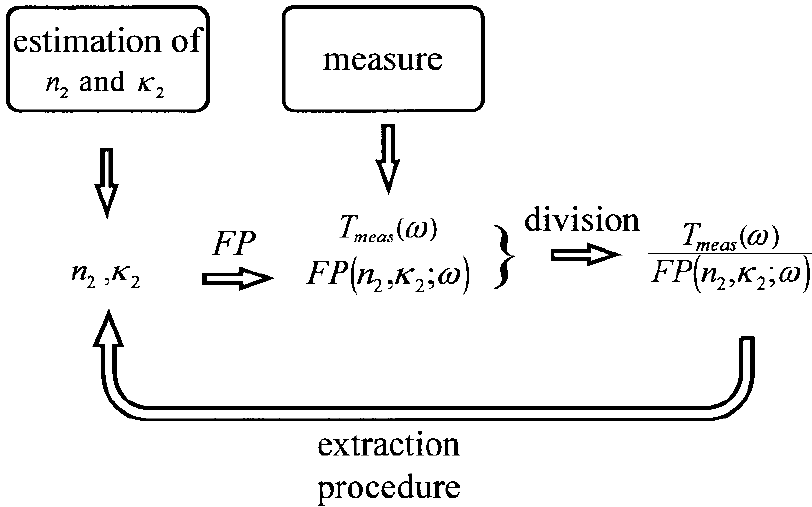
\includegraphics[width=0.5\textwidth]{images/procedure_fp.jpg}
        \caption{The schematic procedure of extracting the refractive index from thin samples. Note that $n_2, \kappa_2$ are the refractive indices.}
      \end{figure}
      \textcolor{tugreen}{A Reliable Method for Extraction of Material Parameters in Terahertz Time-Domain Spectroscopy} from Lionel Duvillaret, Frédéric Garet, and Jean-Louis Coutaz,IEEE \textbf{2} (1996).
  \end{column}
\end{columns}

\end{frame}


%\begin{frame}{2D-Materials}
%  The last "challenge": Thin materials.
%  Substrate influences the measurment.
%  The result is a signal from the substrate and a very weak signal from the 2D-material.
%  \begin{figure}
%    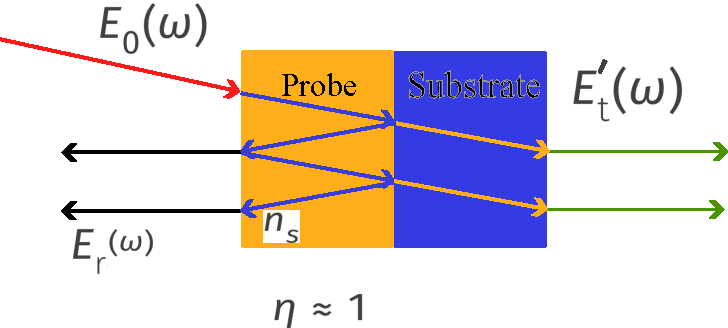
\includegraphics[width=0.5\textwidth]{images/2d.pdf}
%    \caption{The Probe is applied onto a substrate that also alters the intial THz-wave.}
%  \end{figure}
%\end{frame}
%
%\begin{frame}
%  For this we have to consider the transmission coeffiecients $t(\omega)$ of both mediums.
%  Aswell as reflections inside the medium.
%  We can write the transmitted THz-wave as
%  \begin{equation}
%    E_\text{t} '(\omega) = \eta t_\text{Probe}(\omega) t_\text{Sub}(\omega)FP(\omega)E_0(\omega)
%  \end{equation}
%  where $t_\text{Probe}(\omega)$ and $t_\text{Sub}(\omega)$ denote the transmission coeffiecients of the probe and substrate respectively.
%  The complex transfer function $H_0'$ can then be writen as 
%  \begin{equation}
%    H_0(\omega) = \frac{2 n_s(n_\text{sub} + 1)}{(n_\text{s} + n_\text{sub})(n_s + 1)} \symup{exp}\left[ - i (n_s - 1) \frac{\omega l }{c}\right]
%  \end{equation}
%  \textcolor{tugreen}{Time-Resolved Terahertz Spectroscopy Studies on 2D Van der Waals Materials} from Peng Han, Adv. Opt. Mater. \textbf{8} (2020).
%\end{frame}
%
\section{conclusion}
\begin{frame}{Refractive index}
  \begin{center}
  \textcolor{tugreen}{conclusion:}
  This scheme gives an easy way to determine the refractive index of thick homogenous probes through time resolved THz-Spectroscopy.
  It can be extended to also take reflections inside the probe into account by using the Fabry-Perot factor in the transmitted wave.
  However, for most experimental setups this wont be necessary as the post-pulse is sufficiently delayed.\\
  \textcolor{tugreen}{outlook:}
  Numerical Processes can be used to make the scheme even more accurate and take refelections into account aswell.
\end{center}
\end{frame}

\begin{frame}
  \begin{center}
    \begin{columns}
      \begin{column}{0.5\textwidth}
        \begin{figure}
        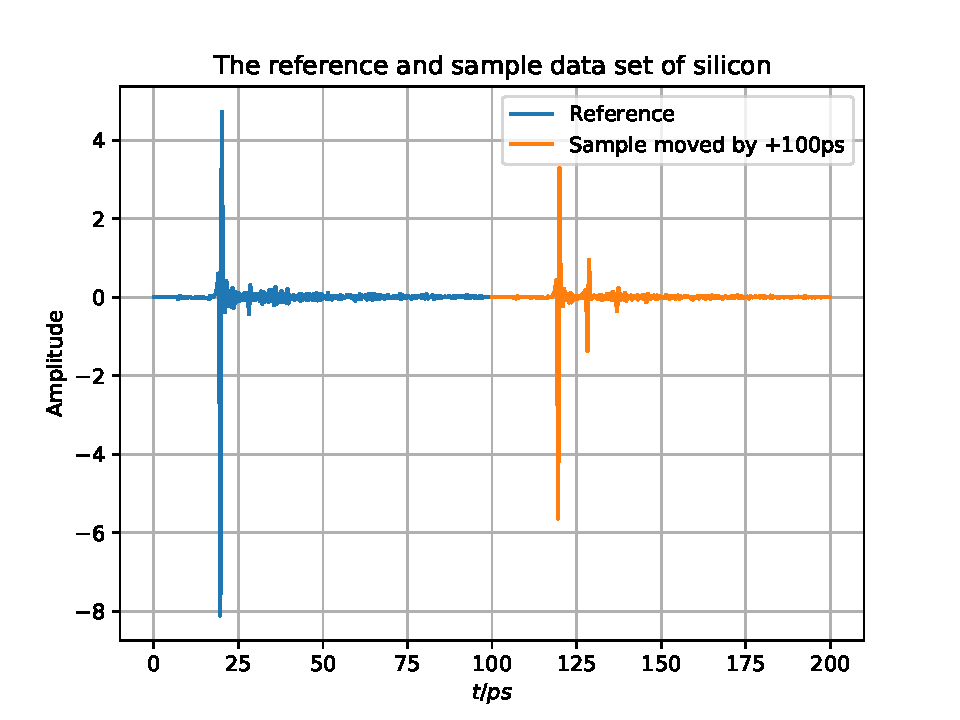
\includegraphics[width=\textwidth]{silicon/THz_timedomain.pdf}
        \caption{Time domain data of silicon}
        \end{figure}
      \end{column}
      \begin{column}{0.5\textwidth}
        \begin{figure}
        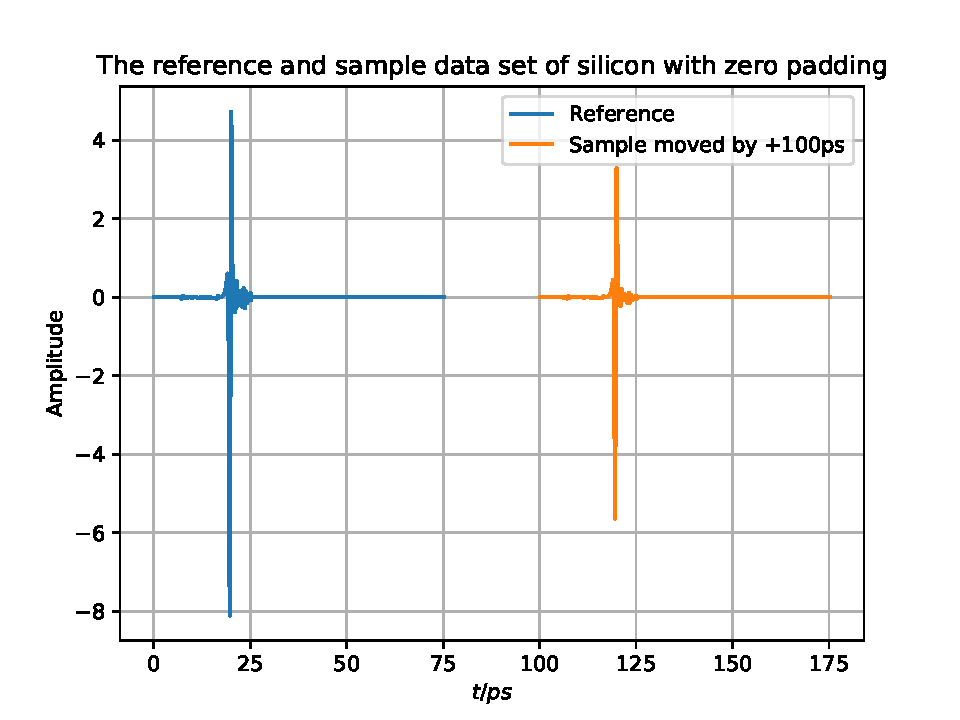
\includegraphics[width=\textwidth]{silicon/THz_timedomain_zero.pdf}
        \caption{Zero padded time domain data of silicon}
        \end{figure}
      \end{column}
    \end{columns}
  \end{center}
\end{frame}

\begin{frame}
  \begin{center}
    \begin{columns}
      \begin{column}{0.5\textwidth}
        \begin{figure}
        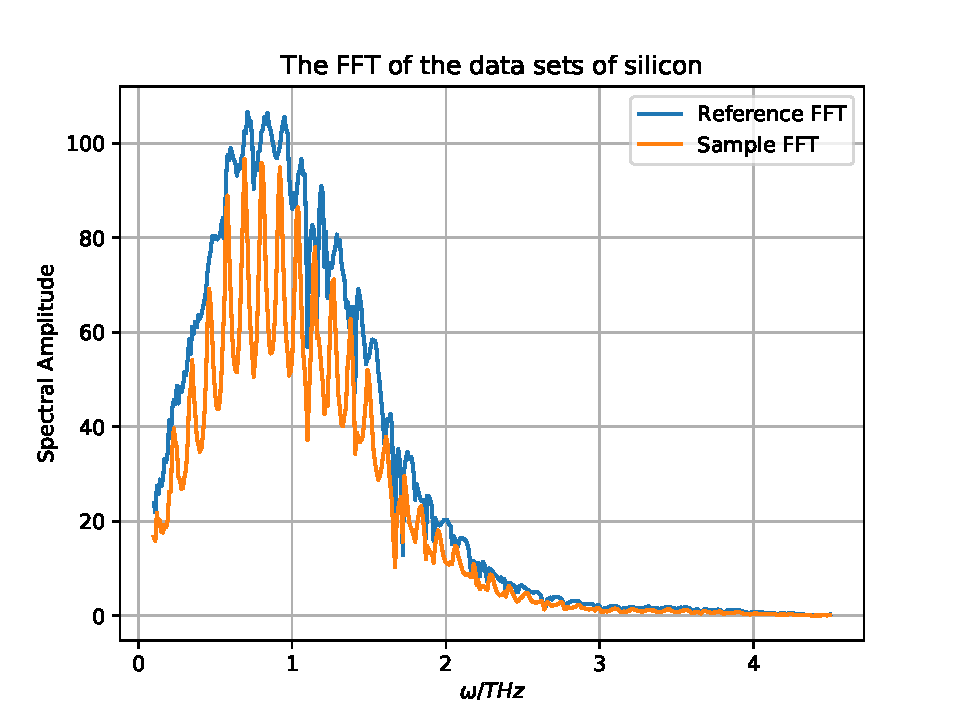
\includegraphics[width=\textwidth]{silicon/THz_FFT.pdf}
        \caption{FFT of the time domain data of silicon}
        \end{figure}
      \end{column}
      \begin{column}{0.5\textwidth}
        \begin{figure}
        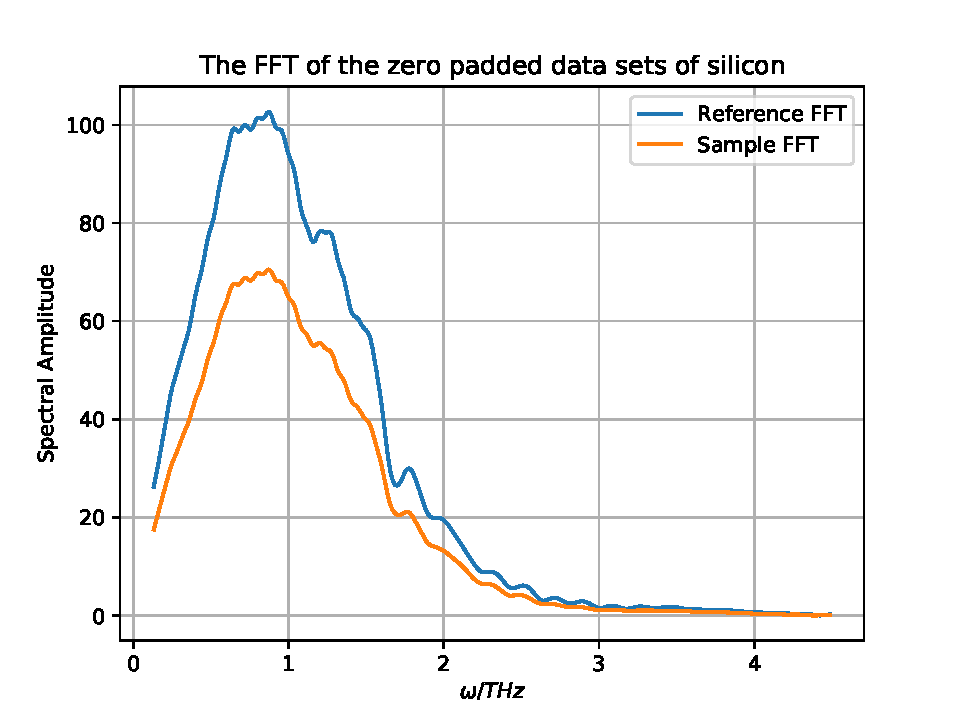
\includegraphics[width=\textwidth]{silicon/THz_FFT_zero.pdf}
        \caption{FFT of the zero padded time domain data of silicon}
        \end{figure}
      \end{column}
    \end{columns}
  \end{center}
\end{frame}

\begin{frame}
  \begin{center}
    \begin{columns}
      \begin{column}{0.5\textwidth}
        \begin{figure}
        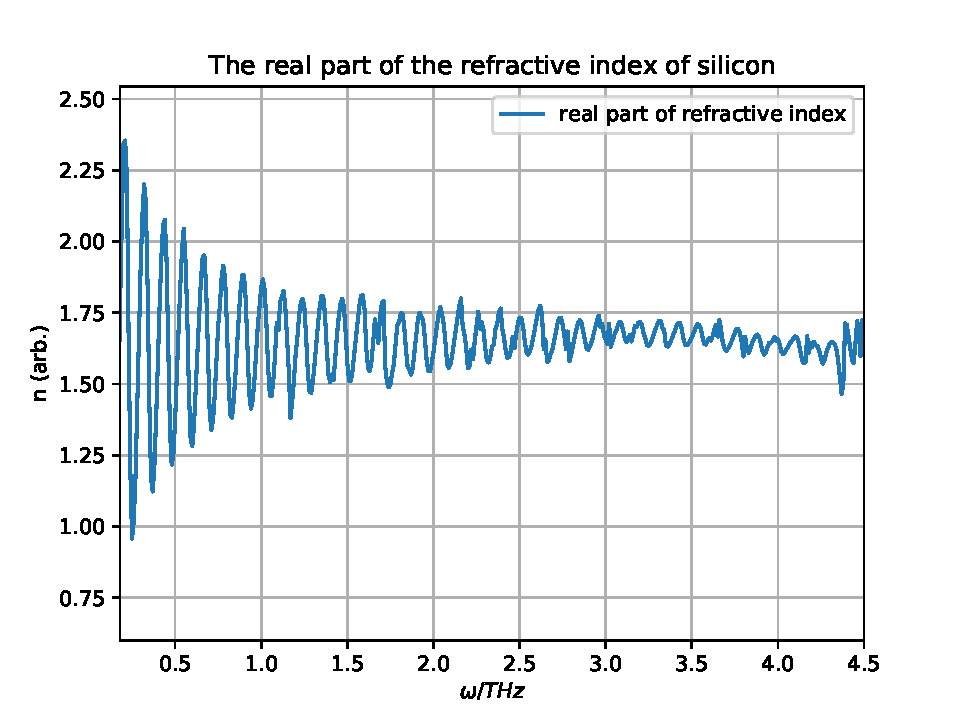
\includegraphics[width=\textwidth]{silicon/THz_real_index.pdf}
        \caption{Real part of the refractive index of silicon}
        \end{figure}
      \end{column}
      \begin{column}{0.5\textwidth}
        \begin{figure}
        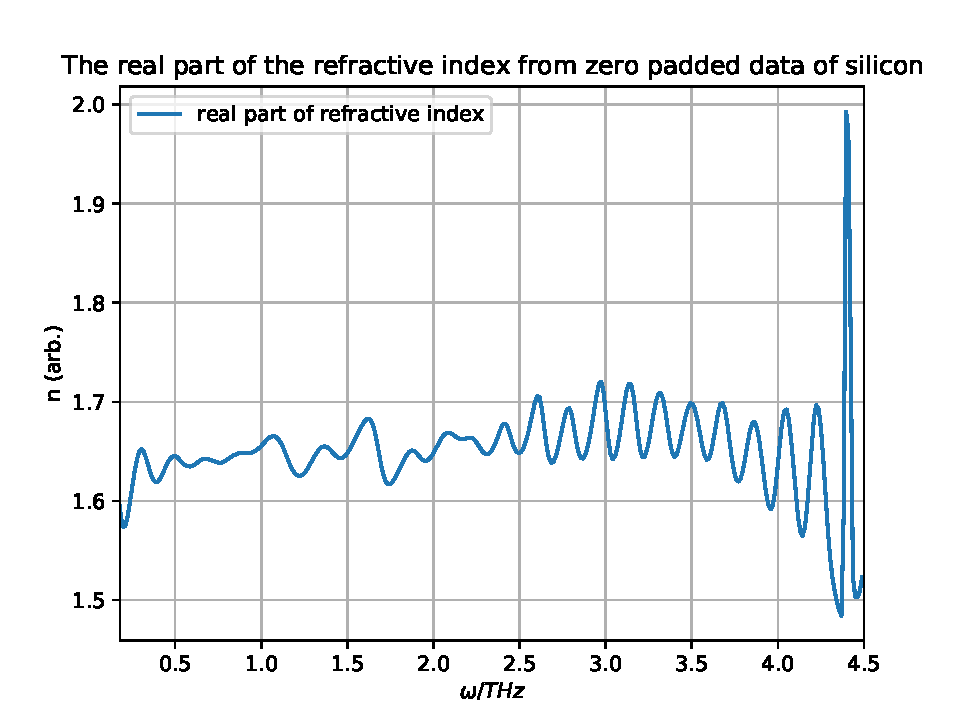
\includegraphics[width=\textwidth]{silicon/THz_real_index_zero.pdf}
        \caption{Real part of the refractive index of silicion with zero padding}
        \end{figure}
      \end{column}
    \end{columns}
  \end{center}
\end{frame}

\begin{frame}
  \begin{center}
    \begin{columns}
      \begin{column}{0.5\textwidth}
        \begin{figure}
        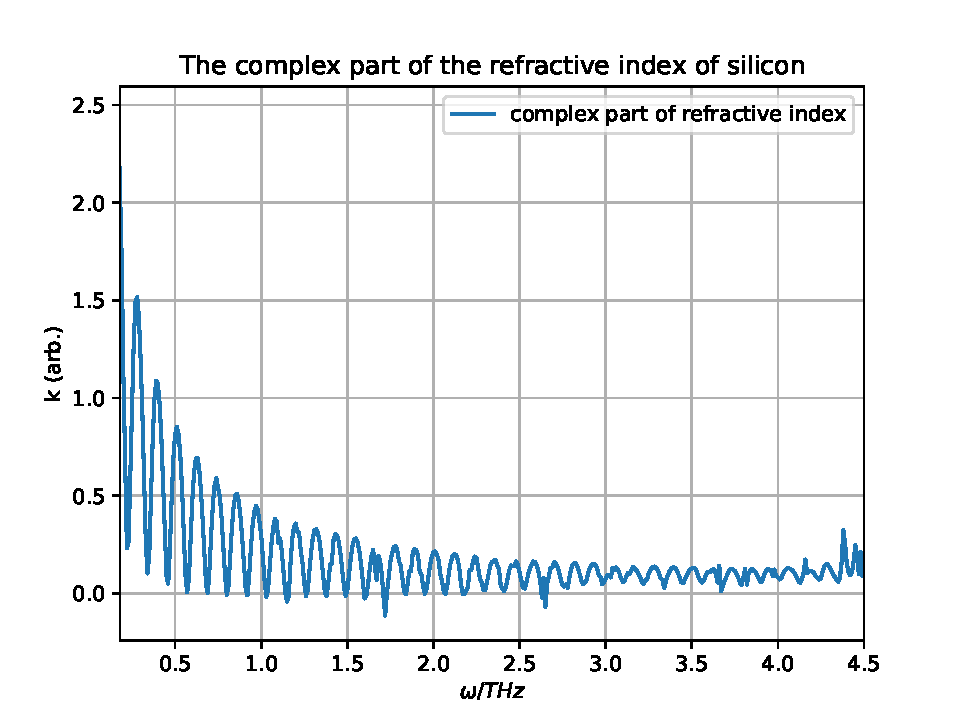
\includegraphics[width=\textwidth]{silicon/THz_complex_index.pdf}
        \caption{The complex part of the refractive index of silicon}
        \end{figure}
      \end{column}
      \begin{column}{0.5\textwidth}
        \begin{figure}
        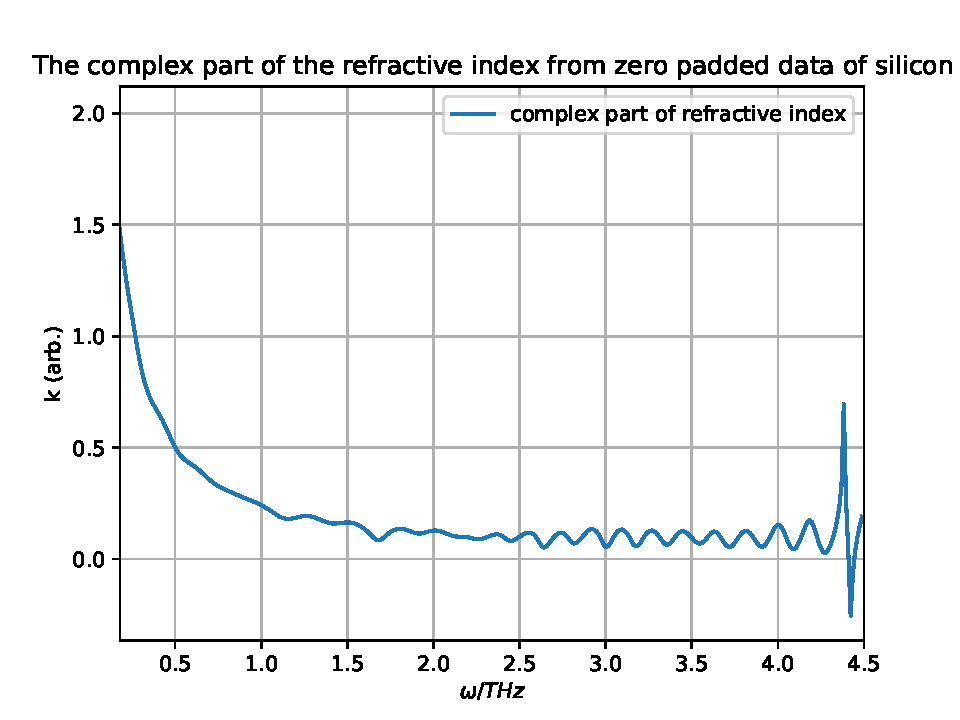
\includegraphics[width=\textwidth]{silicon/THz_complex_index_zero.pdf}
        \caption{The real part of the refractive index of silicon with zero padding}
        \end{figure}
      \end{column}
    \end{columns}
  \end{center}
\end{frame}

\begin{frame}
  \begin{center}
    \begin{columns}
      \begin{column}{0.5\textwidth}
        \begin{figure}
        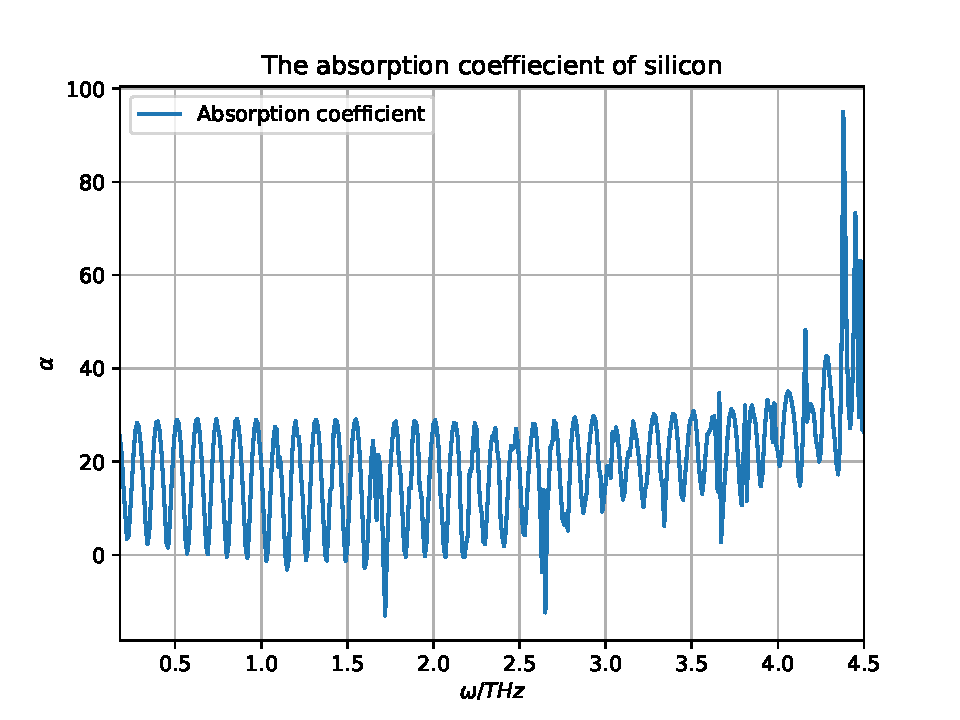
\includegraphics[width=\textwidth]{silicon/THz_absorption.pdf}
        \caption{The absorption coeffiecient of silcion}
        \end{figure}
      \end{column}
      \begin{column}{0.5\textwidth}
        \begin{figure}
        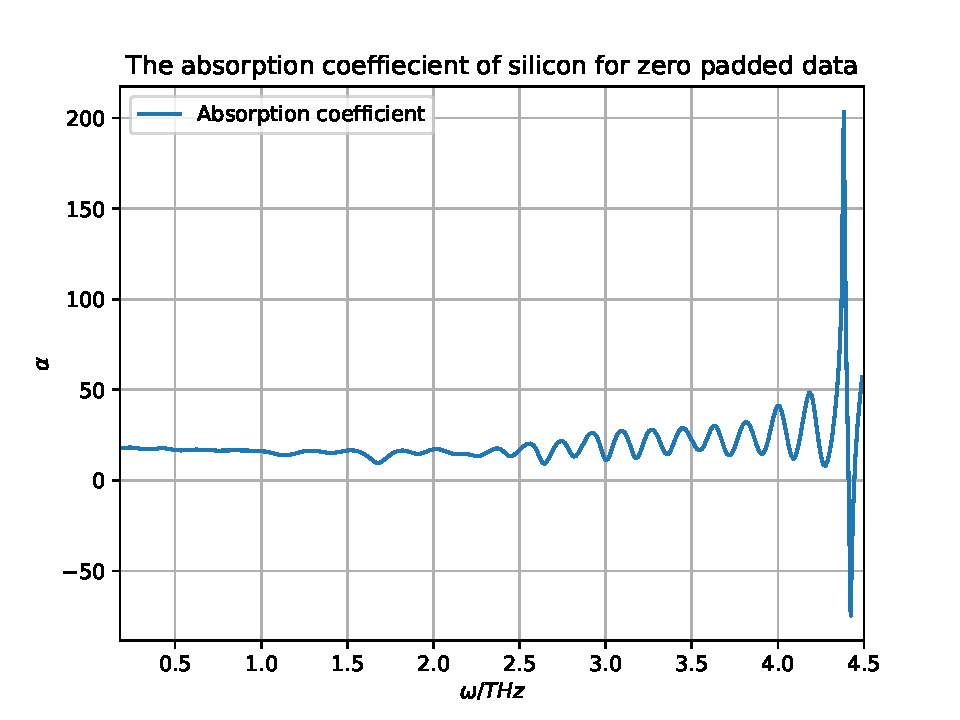
\includegraphics[width=\textwidth]{silicon/THz_absorption_zero.pdf}
        \caption{The absorption coeffiecient of silicion with zero padding}
        \end{figure}
      \end{column}
    \end{columns}
  \end{center}
\end{frame}


\end{document} 